\section{Auswertung}
\label{sec:Auswertung}

\subsection{Bestimmung der Apparatenkonstante}
\label{sec:Apparatenkonstante}
Um die Apparatenkonstante zu bestimmen, werden die Dichten der Kugeln benötigt.
Die Messwerte der Massen und Radien der beiden Kugeln sind in Tabelle \ref{tab:MasseundDichte} zu finden.
Die Radien und Massen bestimmen sich zu
\begin{align*}
  r_{\symup{Gr}} &= (7,86 \pm 0,04)\cdot 10^{-3} \,\si{\meter}\\
  m_{\symup{Gr}} &= (4,54 \pm 0,01) \cdot 10^{-3} \,\si{\kilo\gram}\\
  r_{\symup{Kl}} &= (7,64 \pm 0,11)\cdot 10^{-3} \,\si{\meter}\\
  m_{\symup{Kl}} &= (4,44 \pm 0,02) \cdot 10^{-3} \,\si{\kilo\gram}.\\
\end{align*}

Aus () ergibt sich für die Dichten
\begin{align*}
  \rho_{\symup{Gr}} &= (2232 \pm 34) \,\frac{\si{\kg}}{\si{m^3}}  \\
  \rho_{\symup{Kl}} &= (2380 \pm 10) \,\frac{\si{\kg}}{\si{m^3}}. \\
\end{align*}

\begin{table}
  \centering
  \caption{Messdaten der Massen und Radien der beiden Kugeln.}
  \label{tab:MasseundDichte}
  \begin{tabular}{c c c c}
    \toprule
    $r_{\symup{Gr}}/10^{-3}\,\unit{\meter}$ & $m_{\symup{Gr}}/10^{-3}\,\unit{\kilo\gram}$ & $r_{\symup{Kl}}/10^{-3}\,\unit{\meter}$ & $m_{\symup{Kl}}/10^{-3}\,\unit{\kilo\gram}$ \\
    \midrule
    7,90 & 4,54 & 7,75 & 4,46 \\
    7,80 & 4,56 & 7,55 & 4,46 \\
    7,85 & 4,54 & 7,55 & 4,43 \\
    7,90 & 4,54 & 7,80 & 4,42 \\
    7,85 & 4,54 & 7,55 & 4,43 \\
    \bottomrule
  \end{tabular}
\end{table}
Weiterhin werden noch die Fallzeiten der beiden Kugeln im Viskosimeter benötigt.
Die Fallzeiten der kleinen und der großen Kugel sind in Tabelle \ref{tab:Fallzeit} angegeben. Aus den Messwerten ergibt sich für die Fallzeiten
\begin{align*}
  t_{\symup{Kl}} &= (12,04 \pm 0,18)\,\unit{\second} \\
  t_{\symup{Gr}} &= (39,7 \pm 0,39)\,\unit{\second}. \\
\end{align*}

\begin{table}
  \centering
  \caption{Fallzeiten der Kugeln.}
  \label{tab:Fallzeit}
  \begin{tabular}{c c}
    \toprule
    $t_{\symup{Kl}}/\unit{\second} $ & $t_{\symup{Gr}}/\unit{\second}$ \\
    \midrule
    12,28 & 40,17 \\
    12,06 & 40,17 \\
    11,94 & 39,27 \\
    11,97 & 39,67 \\
    12,12 & 39,67 \\
    12,12 & 39,55 \\
    12,13 & 39,40 \\
    11,87 & 39,57 \\
    11,87 & 40,52 \\
    11,59 & 39,85 \\
    12,12 & 39,52 \\
    12,13 & 39,60 \\
    11,88 & 39,43 \\
    11,97 & 39,49 \\
    12,09 & 38,92 \\
    12,47 & 39,09 \\
    12,15 & 40,11 \\
    12,06 & 40,17 \\
    12,06 & 39,99 \\
    11,84 & 39,88 \\
    \bottomrule
  \end{tabular}
\end{table}

Nun wird mit Hilfe der Fallzeitwerte der kleinen Kugel die Viskosität von Wasser bei Raumtemperatur bestimmt. Dabei werden
\begin{align*}
  K_{\symup{Kl}} &= 7,64\cdot 10^{-8} \,\frac{\unit{\pascal}\cdot\unit{\meter^3}}{\unit{\kilo\gram}} \\
  \rho_{\symup{Fl}} &= 998,2\,\frac{\unit{\kilo\gram}}{\unit{\meter^3}}
\end{align*}
verwendet. $K_{\symup{Kl}}$ ist die angegeben Appartenkonstante für die kleine Kugel \cite{anleitung107}  und $\rho_{\symup{Fl}}$
die Dichte von Wasser bei Raumtemperatur \cite{waterdensity}. Daraus ergibt sich für die Viskosität des Wassers bei Raumtemperatur
\begin{align*}
  \eta_{\symup{RT}} = (1,27 \pm 0,02)\cdot 10^{-3} \,\unit{\pascal}\cdot\unit{\second}.
\end{align*}

\begin{figure}
  \centering
  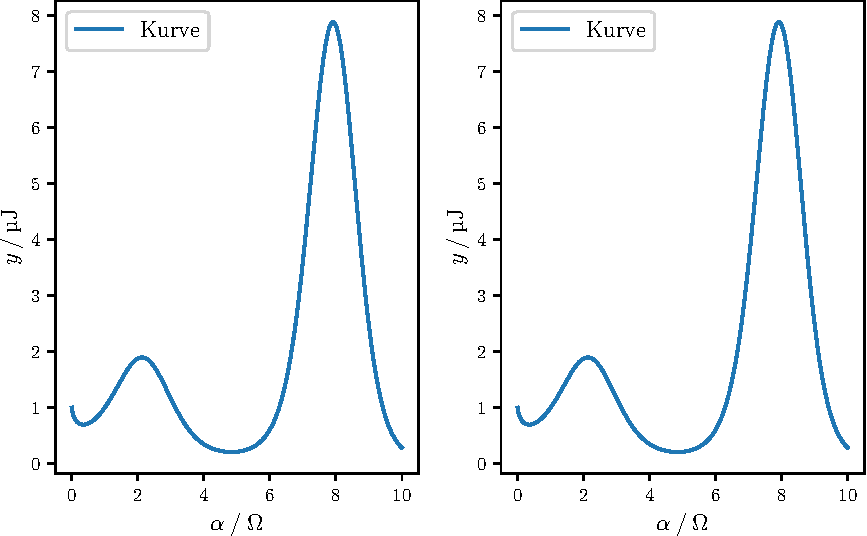
\includegraphics{plot.pdf}
  \caption{Plot.}
  \label{fig:plot}
\end{figure}